%Este trabalho está licenciado sob a Licença Atribuição-CompartilhaIgual 4.0 Internacional Creative Commons. Para visualizar uma cópia desta licença, visite http://creativecommons.org/licenses/by-sa/4.0/deed.pt_BR ou mande uma carta para Creative Commons, PO Box 1866, Mountain View, CA 94042, USA.

\chapter{EDO de primeira ordem}\label{cap_edo1ordem}
\thispagestyle{fancy}

\section{Equação linear}\label{cap_edo1ordem_sec_eqlinear}

A forma geral de uma \emph{EDO linear de primeira ordem} é
\begin{equation}
  P(t)\frac{dy}{dt} + Q(t)y = G(t),
\end{equation}
onde $P(t) \neq 0$, $Q(t)$ e $G(t)$ são funções de $t$. Esta pode ser reescrita na forma
\begin{equation}
  \color{blue}{\frac{dy}{dt} + p(t)y = g(t)},
\end{equation}
escolhendo $p(t) = Q(t)/P(t)$ e $g(t) = G(t)/P(t)$.

\subsection{EDO autônoma e homogênea}

\begin{flushright}
  \href{https://archive.org/details/metodo-de-solucao-edo-ordem-1-linear-coeficientes-constantes-homogenea_20200421}{$\blacktriangleright$ Vídeo disponível!}
\end{flushright}

Primeiramente, vamos considerar o caso em que $p(t) \equiv a \neq 0$ (constante) e $g(t) \equiv 0$, i.e.
\begin{equation}\label{eq:edo1linear_pc_g0}
  \color{blue}{\frac{dy}{dt} + ay = 0.}
\end{equation}
Observamos que $y(t)\equiv 0$ é solução trivial. Agora, para $y(t)\neq 0$, podemos reescrever esta equação da seguinte forma
\begin{align}
  \frac{dy}{dt} &= -ay \\
  \frac{1}{y}\frac{dy}{dt} &= -a
\end{align}
Integrando em relação a $t$, obtemos
\begin{align}
  \int \frac{1}{y}\frac{dy}{dt}\,dt &= -\int a\,dt \\
  \ln|y| &= -at + c \\
  e^{\ln|y|} &= e^{-at + c} \\
  e^{\ln|y|} &= e^{-at}e^c \\
  |y| &= ce^{-at},
\end{align}
onde $c$ é uma constante indeterminada. Da definição do valor absoluto, temos esta última equação nos fornece que
\begin{align}
  y>0 &\Rightarrow y = |y| = ce^{-at}\\
  y<0 &\Rightarrow -y = |y| = ce^{-at}\Rightarrow y=-ce^{-at}.
\end{align}
Lembrando que $c$ é uma constante indeterminada, em qualquer caso, temos
\begin{equation}
  y(t) = ce^{-at}.
\end{equation}
Observamos, ainda, que tomando $c=0$ esta última equação também engloba a solução trivial $y(t)\equiv 0$.

Portanto, concluímos que a \emph{solução geral} de \eqref{eq:edo1linear_pc_g0} é
\begin{equation}
  \color{blue}{y(t) = ce^{-at}.}
\end{equation}

\begin{ex}\label{ex:edo1o_pvi}
  Vamos resolver o seguinte Problema de Valor Inicial (PVI)
  \begin{align}
    &y' - y = 0, \quad t>0,\\
    &y(0) = 1.
  \end{align}
  
  Começamos calculando a solução geral da EDO:
  \begin{align}
    y' &= y\\
    \frac{1}{y}\frac{dy}{dt} &= 1 \\
     \int \frac{1}{y}\frac{dy}{dt}\,dt &= \int 1\,dt \\
       \ln|y| &= t + c \\
    e^{\ln|y|} &= e^{t+c}\\
    y(t) &= ce^{t}.\\
  \end{align}
  Por fim, aplicamos a condição inicial
  \begin{align}
    y(0) &= 1 \\
    ce^{0} &= 1 \\
    c &= 1
  \end{align}
  Concluímos que a solução do PVI é
  \begin{equation}
    y(t) = e^{t}.
  \end{equation}

  \begin{figure}[H]
    \centering
    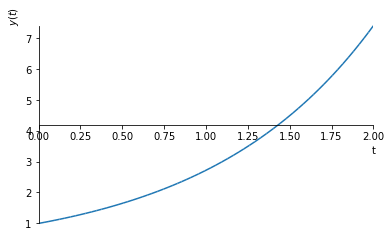
\includegraphics[width=0.7\textwidth]{cap_edo1ordem/dados/fig_ex_edo1o_pvi/fig_ex_edo1o_pvi}
    \caption{Solução do problema de valor inicial tratado no Exemplo \ref{ex:edo1o_pvi}.}
    \label{fig:ex_edo1o_pvi}
  \end{figure}

  \ifispython
  No \python, podemos computar a solução solução geral da EDO com os seguintes comandos:
\begin{verbatim}
In : t = symbols('t')
In : y = symbols('y', cls=Function)
In : edo = Eq(y(t).diff(t)-y(t),0)
In : sol = dsolve(edo,y(t))
In : sol
Out: Eq(y(t), C1*exp(t))
\end{verbatim}
Então, para aplicarmos a condição inicial e obtermos a solução do PVI, usamos:
\begin{verbatim}
In : C1 = symbols('C1')
In : cs = solve(Eq(sol.rhs.subs(t,0),1),dict=True)
In : cs
Out: [{C1: 1}]

In : sol = sol.subs(cs[0])
In : sol
Out: Eq(y(t), exp(t))
\end{verbatim}
O esboço do gráfico da solução pode ser produzido com:
\begin{verbatim}
In: plot(sol.rhs, (t,0, 2), ylabel="$y(t)$")
\end{verbatim}
  \fi
\end{ex}

\subsection{Método dos fatores integrantes}

\begin{flushright}
  \href{https://archive.org/details/edo-ordem-1-linear-coeficientes-constantes-nao-homogenea}{$\blacktriangleright$ Vídeo disponível!}
\end{flushright}

Vejamos, agora, o caso de uma EDO da forma
\begin{equation}\label{eq:edo1linear_pa_g}
  \color{blue}{\frac{dy}{dt} + ay = g(t).}
\end{equation}

O \emph{método dos fatores integrantes} consiste em multiplicarmos a equação por uma função $\mu = \mu(t)$ (fator integrante) de forma que
\begin{equation}
  \color{blue}{\mu\frac{dy}{dt} + \mu ay = \frac{d}{dt}\left(\mu y\right).}
\end{equation}
Pela regra do produto para derivada, temos que
\begin{equation}
  \mu\frac{dy}{dt} + \mu ay = \mu\frac{dy}{dt} + \mu'y.
\end{equation}
Ou seja, tal função $\mu$ deve satisfazer a seguinte EDO
\begin{equation}
  \color{blue}{\mu' = a\mu.}
\end{equation}
Usando o mesmo procedimento utilizado para \eqref{eq:edo1linear_pc_g0}, obtemos que
\begin{equation}
  \mu(t) = ce^{at}.
\end{equation}
Observamos que qualquer escolha de $c\neq 0$ é apropriada e, por simplicidade, escolhemos $c=1$. Ou seja, escolhemos o fator integrante
\begin{equation}
  \color{blue}{\mu(t) = e^{at}}.
\end{equation}

Agora, retornamos a equação \eqref{eq:edo1linear_pa_g}. Multiplicando-a pelo fator integrante $\mu(t) = e^{at}$, obtemos
\begin{gather}
  \mu\frac{dy}{dt} + \mu a y = \mu g(t) \\
  \frac{d}{dt}\left(\mu y\right) = \mu g(t) \\
  \int \,d(\mu y) = \int \mu g(t)\,dt \\
  \mu y = \int \mu g(t)\,dt + c \\
  y = \frac{1}{\mu}\left[\int \mu g(t)\,dt + c\right]. \\
\end{gather}
Portanto, concluímos que
\begin{equation}
  \color{blue}{y(t) = e^{-at}\left[\int g(t)e^{at}\,dt + c\right]}
\end{equation}
é a \emph{solução geral} de \eqref{eq:edo1linear_pa_g}.

\begin{ex}
  Vamos calcular a solução geral da seguinte EDO
  \begin{equation}\label{eq:exer_edo1linear_1}
    y' - y = 1. 
  \end{equation}
  Aplicando o método dos fatores integrantes, temos
  \begin{align}
    \mu y' - \mu y &= (\mu y)' \\
                   &= \mu' y + \mu y'.
  \end{align}
  Ou seja, devemos escolher $\mu$ tal que
  \begin{gather}
    \mu' = -\mu \\
    \frac{1}{\mu}\frac{d\mu}{dt} = -1 \\
    \int \frac{1}{\mu}\,d\mu = -\int 1\,d\mu \\
    \ln|\mu| = -t + c \\
    \mu = ce^{-t}
  \end{gather}
  Por simplicidade, escolhemos $\mu = e^{-t}$.

  Com isso, a EDO \eqref{eq:exer_edo1linear_1} pode ser reescrita como
  \begin{gather}
    \frac{d}{dt}\left(\mu y\right) = \mu\cdot 1 \\
    \frac{d}{dt}\left(e^{-t}y\right) = e^{-t}.
  \end{gather}
  Integrando, obtemos
  \begin{gather}
    e^{-t}y = \int e^{-t}\,dt \\
    e^{-t}y(t) = -e^{-t} + c \\
    y(t) = -e^te^{-t} + ce^{t} \\
    y(t) =  -1 + ce^{t},
  \end{gather}
  a qual é a solução geral. A figura abaixo contém esboços dos gráficos da solução geral para diferentes valores de $c$.

  \begin{figure}[H]
    \centering
    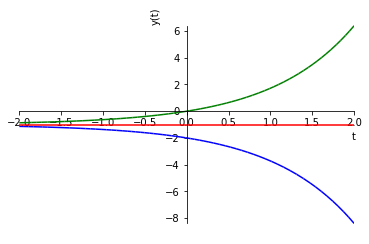
\includegraphics[width=0.7\textwidth]{cap_edo1ordem/dados/fig_ex_edo1o_fi/fig_ex_edo1o_fi}
    \caption[Esboço do gráfico da solução geral para diferentes valores de $c$.]{Esboço do gráfico da solução geral para: (verde) $c=1$, (vermelho) $c=0$ e (azul) $c=-1$.}
    \label{fig:ex_edo1o_fi}
  \end{figure}

  \ifispython
  No \python, podemos computar a solução solução geral da EDO e fazer o gráfico acima com os seguintes comandos:
\begin{verbatim}
In : from sympy import *
In : y = symbols('y', cls=Function)
In : t,C1 = symbols('t,C1')
In : edo = Eq(diff(y(t),t)-y(t),1)
In : sg = dsolve(edo)
In : sg
Out: Eq(y(t), C1*exp(t) - 1)

In : p = plot(sg.rhs.subs(C1,-1), (t,-2,2), \
...:          ylabel="y(t)", line_color="blue", show=False)
...: 
In : q = plot(sg.rhs.subs(C1,0), (t,-2,2), \
...:          ylabel="y(t)", line_color="red", show=False)
...: 
In : p.extend(q)
In : q = plot(sg.rhs.subs(C1,1), (t,-2,2), \
...:          ylabel="y(t)", line_color="green", show=False)
...: 
In : p.extend(q)
In : p.show()
\end{verbatim}
  \fi
\end{ex}

\subsection{Caso geral}

\begin{flushright}
  \href{https://archive.org/details/edo-ordem-1-linear}{$\blacktriangleright$ Vídeo disponível!}
\end{flushright}

O caso geral de uma EDO linear de primeira ordem
\begin{equation}\label{eq:edo1linear_pg}
  \color{blue}{y' + p(t)y = g(t)}
\end{equation}
também pode ser resolvido pelo \emph{método dos fatores integrantes}. Neste caso, o fator integrante $\mu = \mu(t)$ deve ser escolhido de forma que
\begin{align}
  \mu y' + \mu p(t) y &= (\mu y)' \\
                      &= \mu' y + \mu y',
\end{align}
ou seja
\begin{equation}
  \mu' = p(t)\mu.
\end{equation}
Integrando, obtemos o \emph{fator integrante}
\begin{equation}
  \color{blue}{\mu(t) = e^{\int p(t)\,dt}.}
\end{equation}

Usando este fator integrante, a equação \eqref{eq:edo1linear_pg} pode ser reescrita da seguinte maneira
\begin{equation}
  \frac{d}{dt}\left(\mu y\right) = \mu g(t).
\end{equation}
Integrando, obtemos a \emph{solução geral}
\begin{equation}
  \color{blue}{y(t) = \frac{1}{\mu(t)}\left[\int \mu(t) g(t)\,dt + c\right].}
\end{equation}

\begin{ex}
  Vamos calcular a solução geral da seguinte EDO
  \begin{equation}\label{ex:edo1linear_geral}
    y' + \frac{1}{t}y = t.
  \end{equation}

  Primeiramente, calculamos o fator integrante $\mu = \mu(t)$ tal que
  \begin{equation}
    \mu y' + \mu \frac{1}{t} y = (\mu y)' = \mu'y + \mu y'.
  \end{equation}
  Ou seja, precisamos que
  \begin{equation}
    \mu' = \frac{1}{t}\mu.
  \end{equation}
  Integrando, obtemos
  \begin{align}
    \mu(t) &= e^{\int \frac{1}{t}\,dt} \\
           &= e^{\ln|t|} \\
           &= t
  \end{align}

  Aplicando o fator integrante a EDO \eqref{ex:edo1linear_geral}, obtemos
  \begin{gather}
    \frac{d}{dt}\left(t y\right) = t^2 \\
    ty = \int t^2\,dt \\
    y = \frac{1}{t}\left[\frac{t^3}{3} + c\right] \\
    y = \frac{t^2}{3} + \frac{c}{t}
  \end{gather}
\end{ex}

\subsection{Aplicação em modelagem}

\begin{ex}\normalfont{(Mistura em tanque)}
  No instante inicial $t=0$~s (segundo), um tanque contem $q_0$~kg (quilograma) de sal dissolvido em $l$~L (litro) de água. Uma solução de $s$~kg/L de sal e água entra no tanque a uma taxa de $r$~L/s. Esta solução mistura-se com o líquido presente no tanque e a mistura final sai do tanque a mesma taxa de $r$~L/s.

  Vamos modelar a quantidade de sal $q$~kg presente no tanque a cada instante $t$~s. Temos que $q$ é função do tempo $t$~s, i.e. $q = q(t)$. A condição inicial é
  \begin{equation}
    q(0) = q_0.
  \end{equation}
  A taxa de variação de $q$ no tempo é $dq/dt$ e é modelada por
  \begin{equation}
    \frac{dq}{dt} = \underbrace{sr}_{\text{taxa de entrada}} - \underbrace{\frac{q}{l}r}_{\text{taxa de saída}}.
  \end{equation}
  Ou seja, o problema é modelado como o seguinte PVI
  \begin{align}
    &\frac{dq}{dt} = sr - \frac{q}{l}r,\quad t>0,\\
    &q(0) = q_0,
  \end{align}
  onde $s$, $r$, $l$ e $q_0$ são parâmetros do problema. A EDO relacionada é linear de primeira ordem e, portanto, pode ser resolvida pelo método dos fatores integrantes. Veja o Exercício Resolvido \ref{exeresol:mistura_em_tanque}.
\end{ex}

\begin{ex}\normalfont{(Objeto em queda livre)}
  Seja $m$~kg a massa de um objeto em queda livre em um meio com resistência de $\gamma$~kg/s e aceleração da gravidade de $g$~m/s$^2$. A segunda lei de Newton é a lei física que estabelece que a força total atuando sobre o objeto é igual a sua massa multiplicada por sua aceleração. Desta forma, obtemos
  \begin{equation}
    \underbrace{m\frac{dv}{dt}}_{\text{massa}\times\text{aceleração}} = \underbrace{mg}_{\text{força da gravidade}} - \underbrace{\gamma v}_{\text{força da resistência}]},
  \end{equation}
  onde $v = v(t)$~m/s é a velocidade do objeto (sentido positivo igual ao da força da gravidade). Assumindo que o objeto tem velocidade $v_0$~m/s no instante inicial $t=0$, o modelo resume-se ao seguinte PVI:
  \begin{align}
    &m\frac{dv}{dt} = mg - \gamma v,\quad t>0, \\
    &v(0) = v_0,
  \end{align}
  onde $m$, $g$, $\gamma$ e $v_0$ são parâmetros.
\end{ex}

\subsection*{Exercícios resolvidos}

\begin{exeresol}
  Resolva o seguinte PVI
  \begin{align}
    &y' + y = 1, \quad t>0,\\
    &y(0) = 2.
  \end{align}
\end{exeresol}
\begin{resol}
  Primeiramente, obtemos a solução geral da EDO pelo método dos fatores integrante. Para tanto, buscamos pelo fator integrante $\mu$ tal que
  \begin{equation}
    \mu y' + \mu y = (\mu y)',
  \end{equation}
  ou seja,
  \begin{gather}
    \mu' = \mu \\
    \mu(t) = e^{t}.
  \end{gather}
  Obtido o fator integrante, reescrevemos a EDO como segue
  \begin{gather}
    \frac{d}{dt}\left(\mu y\right) = \mu\cdot 1 \\
    \frac{d}{dt}\left(e^ty\right) = e^t.
  \end{gather}
  Integrando, obtemos a solução geral
  \begin{equation}
    y = 1 + ce^{-t}.
  \end{equation}

  Aplicando a condição inicial, obtemos
  \begin{gather}
    y(0) = 2 \\
    1 + ce^{-0} = 2 \\
    c = 1.
  \end{gather}

  Concluímos que a solução do PVI é $y(t) = 1 + e^{-t}$.
\end{resol}

\begin{exeresol}
  Calcule a solução geral da EDO
  \begin{align}
    y' + \frac{1}{t}y = \sen(t),\quad t>0.
  \end{align}
\end{exeresol}
\begin{resol}
  Buscamos pelo fator integrante $\mu$ tal que
  \begin{equation}
    \mu y' + \mu \frac{1}{t}y = (\mu y)',
  \end{equation}
  ou seja,
  \begin{gather}
    \mu' = \frac{\mu}{t} \\
    \mu(t) = e^{\int \frac{1}{t}\,dt} = e^{\ln|t|} = t.
  \end{gather}
  Obtido o fator integrante, reescrevemos a EDO como segue
  \begin{gather}
    \frac{d}{dt}\left(\mu y\right) = \mu\cdot \sen(t) \\
    \frac{d}{dt}\left(t y\right) = t\sen(t).
  \end{gather}
  Integrando, obtemos a solução geral
  \begin{equation}
    y(t) = \frac{c}{t}  + \frac{\sen(t)}{t} - \cos(t).
  \end{equation}
\end{resol}

\begin{exeresol}(Mistura em tanque)\label{exeresol:mistura_em_tanque}
  No instante inicial $t=0$~s (segundo), um tanque contem $100$~kg de sal dissolvidos em $1000$~L d'água. Uma solução de $0,2$~kg/L de sal e água entra no tanque a uma taxa de $10$~L/s. Esta solução mistura-se com o líquido presente no tanque e a mistura final sai do tanque a mesma taxa de $10$~L/s. Calcule a quantidade de sal misturado no tanque após $1$ hora de operação, i.e. quando $t=3600$~s.
\end{exeresol}
\begin{resol}
  Denotando por $q = q(t)$~kg a quantidade de sal misturado no tanque no instante $t$, temos que a taxa de variação de $q$ no tempo é dada por
  \begin{align}
    \frac{dq}{dt} &= 0,2\cdot 10 - \frac{q}{1000}\cdot 10 \\
                  &= 2 - \frac{q}{100}.
  \end{align}
  Ou seja, o modelo constitui-se no seguinte PVI
  \begin{align}
    \frac{dq}{dt} = 2 - \frac{q}{100},\quad t>0,\label{eq:exeresol_mistura_edo}\\
    q(0) = 100.
  \end{align}

  Para resolver o problema, vamos usar o método dos fatores integrantes. O fator integrante é escolhido como sendo
  \begin{align}
    \mu(t) &= e^{\int \frac{1}{100}\,dt} \\
           &= e^{t/100}.
  \end{align}
  Segue que a EDO \eqref{eq:exeresol_mistura_edo} pode ser reescrita como
  \begin{equation}
    \frac{d}{dt}\left(qe^{t/100}\right) = 2e^{t/100}.
  \end{equation}
  Integrando, obtemos
  \begin{align}
    q(t) &= e^{-t/100}\int 2e^{t/100}\,dt \\
         &= e^{-t/100}\left(200e^{t/100} + c\right) \\
         &= 200 + ce^{-t/100}.
  \end{align}
  Da condição inicial, obtemos
  \begin{gather}
    q(0) = 100 \\
    200 + c = 100 \\
    c = -100.
  \end{gather}
  Logo, a solução do PVI é
  \begin{equation}
    q(t) = 200 - 100e^{-t/100}.
  \end{equation}
  No tempo $t=3600$~s, temos
  \begin{equation}
    q(3600) = 200 - 100e^{-3600/100} \approx 200~\text{kg}.
  \end{equation}
\end{resol}

\subsection*{Exercícios}

\begin{exer}
  Calcule a solução do seguinte PVI
  \begin{align}
    &y' + y = 0, \quad t>0, \\
    &y(0) = 1.    
  \end{align}
\end{exer}
\begin{resp}
  $y(t) = e^{-t}$
\end{resp}

\begin{exer}
  Calcule a solução do seguinte PVI
  \begin{align}
    &y' - y = 2, \quad t>0, \\
    &y(0) = 1.    
  \end{align}
\end{exer}
\begin{resp}
  $y(t) = 3e^{t}-2$
\end{resp}

\begin{exer}
  Calcule a solução geral da seguinte EDO
  \begin{equation}
    y' + y = \sen(t).
  \end{equation}
\end{exer}
\begin{resp}
  $y(t) = ce^{-t} + \frac{\sen(x)}{2} - \frac{\cos(x)}{2}$
\end{resp}

\begin{exer}
  Calcule a solução geral do seguinte PVI
  \begin{align}
    &y' + \frac{1}{t}y = 2t,\quad t>1,\\
    &y(1) = 0.
  \end{align}
\end{exer}
\begin{resp}
  $y(t) = \frac{2}{3}\left(t^2 - \frac{1}{t}\right)$
\end{resp}

\begin{exer}
  Calcule a solução geral do seguinte PVI
  \begin{align}
    &ty' + 2y = 1,\quad t>1,\\
    &y(1) = 1.
  \end{align}
\end{exer}
\begin{resp}
  $y(t) = \frac{1}{2}\left(\frac{1}{t^2} + 1\right)$
\end{resp}

\begin{exer}
  Seja um objeto de massa $m = 1$~kg em queda livre sujeito a aceleração da gravidade de $9,8$~m/s$^2$ e resistência do meio de $\gamma = 0,2$~kg/s. Assuma, ainda, que o objeto está em repouso no tempo inicial e a uma altura de $10$~m (metros) do solo. Quanto tempo leva para o objeto atingir o solo.
\end{exer}
\begin{resp}
  $1.5$~s
\end{resp}

\section{Equação separável}\label{cap_edo1ordem_sec_eqsep}

\begin{flushright}
  \href{https://archive.org/details/edo-ordem-1-separavel}{$\blacktriangleright$ Vídeo disponível!}
\end{flushright}

Uma EDO de primeira ordem
\begin{equation}
  \frac{dy}{dx} = f(x,y)
\end{equation}
é dita ser uma \emph{equação separável} quando pode ser reescrita na seguinte forma
\begin{equation}\label{eq:def_edo_sep}
  {\color{blue} M(x) + N(y)\frac{dy}{dx} = 0.}
\end{equation}

\begin{ex}\label{ex:edo_sep_def}
  Vejamos os seguintes casos.
  \begin{enumerate}[a)]
  \item É separável a EDO
    \begin{equation}
      \frac{dy}{dx} = \frac{x^2}{y},
    \end{equation}
    pois pode ser reescrita como segue
    \begin{gather}
      \frac{dy}{dx} = \frac{x^2}{y} \\
      y\frac{dy}{dx} = x^2 \\
      \underbrace{-x^2}_{M(x)} + \underbrace{y}_{N(y)}\frac{dy}{dx} = 0.
    \end{gather}
  \item Não é separável a EDO
    \begin{equation}
      e^{xy} - x\frac{dy}{dx} = 0.
    \end{equation}
    Observe que não há como reescrever esta equação na forma \eqref{eq:def_edo_sep}.
  \end{enumerate}
\end{ex}

Agora, vamos ver como podemos resolver uma EDO separável. Consideremos a equação separável
\begin{equation}\label{eq:edo_sep_aux}
  M(x) + N(y)\frac{dy}{dx} = 0.
\end{equation}
Sejam, também, $F=F(x)$ e $G=G(y)$ primitivas de $M$ e $N$, respectivamente. I.e.
\begin{align}
  &\frac{d}{dx}F(x) = M(x),\\
  &\frac{d}{dy}G(y) = N(y).
\end{align}
Lembrando que $y = y(x)$, temos da \emph{regra da cadeia} que
\begin{align}
  \frac{d}{dx}G(y) &= \frac{d G(y)}{dy}\frac{dy}{dx} \\
                   &= N(y)\frac{dy}{dx}.
\end{align}
Ou seja, a EDO \eqref{eq:edo_sep_aux} pode ser reescrita na forma
\begin{equation}
  \frac{d}{dx}F(x) + \frac{d}{dx}G(y) = 0
\end{equation}
ou ainda,
\begin{equation}
  \frac{d}{dx}\left(F(x) + G(y)\right) = 0.
\end{equation}
Então, integrando em relação a $x$, obtemos
\begin{equation}
  F(x) + G(y) = c,
\end{equation}
a qual é uma equação algébrica para $y$ que, com sorte, pode ser usada para explicitar a solução da EDO \eqref{eq:edo_sep_aux}.

\begin{ex}\label{ex:edo_sep_metsol}
  Vamos resolver a seguinte EDO separável:
  \begin{equation}
    \frac{dy}{dx} = \frac{x^2}{y}.
  \end{equation}
  \begin{enumerate}[a)]
  \item \emph{Método 1}.
  Primeiramente, reescrevemos a EDO no formato \eqref{eq:def_edo_sep}:
  \begin{equation}
    \underbrace{-x^2}_{M(x)} + \underbrace{y}_{N(y)}\frac{dy}{dx} = 0.
  \end{equation}
  Então, calculamos as primitivas
  \begin{align}
    F(x) &= \int M(x)\,dx\\
         &= \int -x^2\,dx \\
         &= -\frac{x^3}{3} + c
  \end{align}
  e
  \begin{align}
    G(y) &= \int N(y)\,dy \\
         &= \int y\,dy \\
         &= \frac{y^2}{2} + c.
  \end{align}
  Então, segue que a EDO resume-se a seguinte equação algébrica
  \begin{gather}
    F(x) + G(y) = c \\
    -\frac{x^3}{3} + \frac{y^2}{2} = c \label{eq:ex_edo_sep_met1}
  \end{gather}
  a qual é uma equação implícita da solução geral $y = y(x)$. 
  
\item \emph{Método 2}.
  A EDO separável
  \begin{equation}
    \frac{dy}{dx} = \frac{x^2}{y}
  \end{equation}
  pode ser reescrita como
  \begin{equation}
    y\,dy = x^2\,dx.
  \end{equation}
  Integrando ambos os lados desta equação, obtemos
  \begin{equation}
    \frac{y^2}{2} = \frac{x^3}{3} + c,
  \end{equation}
  a qual é equivalente a solução obtida em \eqref{eq:ex_edo_sep_met1}.
\end{enumerate}

Na figura abaixo, temos esboços dos gráficos da solução para diferentes valores de $c$.

\begin{figure}[H]
  \centering
  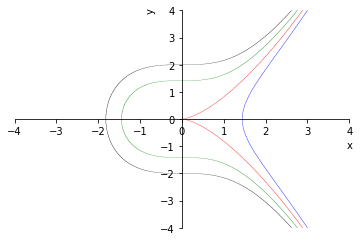
\includegraphics[width=0.6\textwidth]{cap_edo1ordem/dados/fig_ex_edo_sep_metsol/fig_ex_edo_sep_metsol}
  \caption{Esboços dos gráficos da solução da EDO do Exemplo \ref{ex:edo_sep_metsol} para: (azul) $c=-1$, (vermelho) $c=0$, (verde) $c=1$ e (preto) $c=2$.}
  \label{fig:ex_edo_sep_metsol}
\end{figure}

\ifispython
No \python, podemos computar a solução com os seguintes comandos:
\begin{verbatim}
In : from sympy import *
...: y = symbols('y', cls=Function)
...: x,C1 = symbols('x,C1')
...: edo = Eq(diff(y(x),x),x**2/y(x))
...: sg = dsolve(edo, y(x), simplify=False)
...: sg
Out: Eq(y(x)**2/2, C1 + x**3/3)
\end{verbatim}
Os esboços dos gráficos podem ser feitos com:
\begin{verbatim}
In : var('y')
...: sg = sg.subs(y(x),y)
...: p = plot_implicit(sg.subs(C1,-1), (x,-4,4), \
...:          (y,-4,4), line_color="blue", show=False)
...: q = plot_implicit(sg.subs(C1,0), (x,-4,4), \
...:          (y,-4,4), line_color="red", show=False)
...: p.extend(q)
...: q = plot_implicit(sg.subs(C1,1), (x,-4,4), \
...:          (y,-4,4), line_color="green", show=False)
...: p.extend(q)
...: q = plot_implicit(sg.subs(C1,2), (x,-4,4), \
...:          (y,-4,4), line_color="black", show=False)
...: p.extend(q)
...: p.show()
\end{verbatim}
\fi

\end{ex}

\begin{obs}
  Como vimos no exemplo anterior (Exemplo \ref{ex:edo_sep_metsol}), a solução geral de uma EDO separável nem sempre pode ser explicitada. Em muitos casos o procedimento de separar as variáveis nos leva a obter a solução da EDO na forma de uma equação algébrica implícita.
\end{obs}

\subsection{Equação de Verhulst}

A \emph{equação de Verhulst}\footnote{Pierre François Verhulst, 1804-1849, matemático belga.} (ou \emph{equação logística}) é um clássico modelo de crescimento populacional. Trata-se da seguinte equação autônoma
\begin{equation}\label{eq:Verhulst}
  {\color{blue}\frac{dy}{dt} = r\left(1 - \frac{y}{K}\right)y},
\end{equation}
onde $y$ é a medida de tamanho da população e os parâmetros são: $r>0$ a taxa de crescimento intrínseca e $K>0$ o nível de saturação.

Antes de resolvermos esta equação, vamos fazer algumas observações que podem ser obtidas diretamente da EDO. Do cálculo, temos que se $dy/dt = 0$ para todos os valores de $t$, então $y$ é constante, i.e. a população se mantém constante. A derivada é nula quando o lado direito de \eqref{eq:Verhulst} for nulo, i.e.
\begin{equation}
  r\left(1 - \frac{y}{K}\right)y = 0.
\end{equation}
Isso ocorre quando $y = 0$ ou quando $y=K$. Ou seja, se a população é nula não há crescimento populacional, bem como, não há crescimento se a população estiver em seu nível de saturação.

Agora, o que ocorre se a população for $0 < y < K$? Neste caso, temos
\begin{equation}
  \frac{dy}{dt} = r\underbrace{\left(1 - \frac{y}{K}\right)}_{>0}y > 0,
\end{equation}
ou seja, a população cresce. Por outro lado, se $y > K$ (a população está acima de seu nível de saturação), então
\begin{equation}
  \frac{dy}{dt} = r\underbrace{\left(1 - \frac{y}{K}\right)}_{<0}y < 0,
\end{equation}
a população decresce. Estas conclusões também nos levam a inferir que
\begin{equation}
  \lim_{t\to\infty} y(t) = K,
\end{equation}
para qualquer população inicial não nula.

\subsubsection{Solução da equação logística}

Consideramos o seguinte PVI
\begin{align}
  &\frac{dy}{dt} = r\left(1 - \frac{y}{K}\right)y,\quad t>0,\\
  &y(0) = y_0.
\end{align}

A equação de Verhulst é uma EDO separável, daí segue que
\begin{gather}
  \frac{dy}{dt} = r\left(1 - \frac{y}{K}\right)y \\
  \frac{1}{\left(1 - \frac{y}{K}\right)y}\,dy = r\,dt.
\end{gather}
Vamos integrar o lado esquerdo desta última equação\footnote{Vamos usar de decomposição em frações parciais.}
\begin{align}
  \int \frac{1}{\left(1 - \frac{y}{K}\right)y}\,dy &= \int \left(\frac{1}{y} + \frac{1/K}{1-y/K}\right)\,dy \\
                                                   &= \ln|y| - \ln\left|1 - \frac{y}{K}\right|.
\end{align}
Logo, a solução da equação logística satisfaz a seguinte equação algébrica
\begin{equation}
  \ln|y| - \ln\left|1 - \frac{y}{K}\right| = rt + c,
\end{equation}
onde $c$ é uma constante a determinar. Antes, observamos que esta equação é equivalente a
\begin{equation}
  \ln\left|\frac{y}{1 - \frac{y}{K}}\right| = rt + c.
\end{equation}
Aplicando a função exponencial, obtemos
\begin{equation}\label{eq:Verhulst_aux}
  \frac{y}{1 - y/K} = ce^{rt}.
\end{equation}
Da condição inicial $y(0) = y_0$, encontramos
\begin{equation}\label{eq:Verhulst_c}
  c = \frac{y_0}{1 - y_0/K}.
\end{equation}
Agora, podemos isolar $y$ em \eqref{eq:Verhulst_aux} como segue: 
\begin{gather}
  y = \left(1-\frac{y}{K}\right)ce^{rt}\\
  y = ce^{rt} - y\frac{c}{K}e^{rt} \\
  \left(1 + \frac{c}{K}e^{rt}\right)y = ce^{rt}\\
  y = \frac{ce^{rt}}{1+\frac{c}{K}e^{rt}}
\end{gather}
Então, multiplicando em cima e em baixo por $(K/c)e^{-rt}$, obtemos
\begin{equation}
  y = \frac{K}{\frac{K}{c}e^{-rt} + 1}.
\end{equation}
Por fim, de \eqref{eq:Verhulst_c}, obtemos a solução
\begin{equation}\label{eq:sol_verhulst}
  y(t) = \frac{y_0K}{y_0 + (K-y_0)e^{-rt}}.
\end{equation}

Da solução, corroboramos que a população permanece constante quando $y_0 = 0$ ou $y_0 = K$. Ainda, se $0<y_0<K$ ou $y_0 > K$, temos que
\begin{align}
  \lim_{t\to\infty} y(t) &= \lim_{t\to\infty} \frac{y_0K}{y_0 + (K-y_0)\cancelto{0}{e^{-rt}}} \\
                         &= K.
\end{align}

\begin{ex}\label{ex:Verhulst}
Vamos usar a equação de Verhulst para modelar a dinâmica de uma população com taxa de crescimento intrínseca $r=0,1$ e nível de saturação $K=1$ (bilhão). Pelo que vimos nesta subsecção, temos o modelo
\begin{align}
  &\frac{dy}{dt} = 0,1\left(1 - y\right)y,\quad t>0,\\
  &y(0) = y_0,
\end{align}
onde $y:\mapsto y(t)$ é a solução no tempo $t$ e $y_0$ é a população inicial.

De \ref{eq:sol_verhulst}, temos a solução
\begin{equation}
  y(t) = \frac{y_0}{y_0 + (1-y_0)e^{-0,1t}}.
\end{equation}
A figura abaixo, mostra a dinâmica da população para $y_0=0,5<K$, $y_0=1=K$ e $y_0=1,5>K$.

\begin{figure}[H]
  \centering
  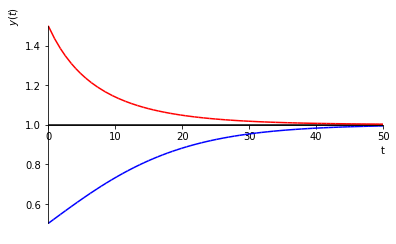
\includegraphics[width=0.7\textwidth]{cap_edo1ordem/dados/fig_ex_Verhulst/fig_ex_Verhulst}
  \caption{Exemplo \ref{ex:Verhulst}. Dinâmicas populacionais para: (azul) $y_0=0,5<K$, (preto) $y=1=K$ e (vermelho) $y=1,5>K$.}
  \label{fig:ex_Verhulst}
\end{figure}
\end{ex}

\subsection*{Exercícios resolvidos}

\begin{exeresol} (\href{https://archive.org/details/er-edo-eq-separavel}{$\blacktriangleright$ Vídeo disponível!})
  
  Calcule a solução geral da EDO
  \begin{equation}
    y' = 2y^2 + xy^2.
  \end{equation}
\end{exeresol}
\begin{resol}
  Separando as variáveis, obtemos
  \begin{gather}
    y' = 2y^2 + xy^2 \\
    \frac{dy}{dx} = y^2(2 + x) \\
    \frac{1}{y^2}\,dy = (2+x)\,dx.
  \end{gather}
  Integrando, obtemos a solução geral
  \begin{align}
    -\frac{1}{y} = 2x + \frac{x^2}{2} + c.
  \end{align}
\end{resol}

\begin{exeresol}
  Calcule a solução do PVI
  \begin{align}
    &\frac{dy}{dx} = \frac{x^2}{y},\quad x>0,\\
    &y(0) = 2.
  \end{align}
\end{exeresol}
\begin{resol}
  Separamos as variáveis e integramos
  \begin{gather}
    \frac{dy}{dx} = \frac{x^2}{y} \\
    y\,dy = x^2\,dx \\
    \int y\,dy = \int x^2\,dx \\
    \frac{y^2}{2} = \frac{x^3}{3} + c.
  \end{gather}
  Determinamos a constante $c$ pela aplicação da condição inicial $y(0) = 2$. Ou seja, temos
  \begin{gather}
    \frac{y^2(0)}{2} = \frac{0^3}{3} + c \\
    c = 2.
  \end{gather}
  Logo, a solução $y = y(x)$ do PVI é dada pela equação algébrica
  \begin{equation}
    \frac{y^2}{2} = \frac{x^3}{3} + 2.
  \end{equation}
  Buscando explicitar a solução, observamos que
  \begin{gather}
    y^2 = \frac{2}{3}x^3 + 4 \\
    y = \pm\sqrt{\frac{2}{3}x^3+4}.
  \end{gather}
  Lembrando que $y(0) = 2$, temos necessariamente que
  \begin{equation}
    y(x) = \sqrt{\frac{2}{3}x^3 + 4}.
  \end{equation}
\end{resol}

\begin{exeresol}(Crescimento populacional com limiar)
  Considere o seguinte modelo de crescimento populacional
  \begin{align*}
    &\frac{dy}{dt} = -r\left(1 - \frac{y}{L}\right)y,\quad t>0,\\
    &y(0) = y_0,
  \end{align*}
  onde $y = y(t)$ é o tamanho da população, $y_0 \geq 0$ é a população inicial e são parâmetros $r, L > 0$. Forneça os valores de $y_0$ para os quais a população é crescente.
\end{exeresol}
\begin{resol}
  A população $y$ é crescente quando
  \begin{equation}
    \frac{dy}{dt} > 0.
  \end{equation}
  Logo, precisamos ter
  \begin{equation}
    -r\left(1 - \frac{y}{L}\right)y > 0.
  \end{equation}
  Isto ocorre quando
  \begin{gather}
    1 - \frac{y}{L} < 0 \\
    y > L.
  \end{gather}
  Logo, concluímos que uma população inicial $y_0 > L$ é necessária para produzir uma taxa de crescimento populacional positiva.
\end{resol}

\subsection*{Exercícios}

\begin{exer}
  Calcule a solução de
  \begin{align}
    \frac{dy}{dx} = xe^y,\quad x>0,\\
    y(0) = 1.
  \end{align}
\end{exer}
\begin{resp}
  $y(x) = \ln\left(\frac{2}{2e^{-1}-x^2}\right)$.
\end{resp}

\begin{exer}
  Resolva a EDO
  \begin{equation}
    y' + y^2\cos x = 0.
  \end{equation}
\end{exer}
\begin{resp}
  $y(x) = \frac{1}{c + \sen x}$
\end{resp}

\begin{exer}
  Resolva o PVI
  \begin{equation}
    e^{x+y}y' = 1,\quad x>0,\\
    y(0) = 0.
  \end{equation}
\end{exer}
\begin{resp}
  $y(x) = \ln\left(2 - e^{-x}\right)$
\end{resp}

\begin{exer}
  Considere o seguinte modelo de crescimento populacional
  \begin{align*}
    &\frac{dy}{dt} = -r\left(1 - \frac{y}{L}\right)y,\quad t>0,\\
    &y(0) = y_0,
  \end{align*}
  onde $y = y(t)$ é o tamanho da população, $y_0 \geq 0$ é a população inicial e são parâmetros $r, L > 0$. Qual é a tendência da população $y = y(t)$ quando $t\to\infty$ e
  \begin{enumerate}[a)]
  \item $y_0 = 0$;
  \item $0 < y_0 < L$;
  \item $y_0 = L$;
  \item $y_0 > L$
  \end{enumerate}
\end{exer}
\begin{resp}
  a)~$y(t) \equiv 0$; b)~$y(t)\to 0$; c)~$y(t)\equiv L$; d)~$y(t)\to\infty$.
\end{resp}

\begin{exer}
  Resolva o seguinte modelo de crescimento populacional
  \begin{align*}
    &\frac{dy}{dt} = -r\left(1 - \frac{y}{L}\right)y,\quad t>0,\\
    &y(0) = y_0,
  \end{align*}
  onde $y = y(t)$ é o tamanho da população, $y_0 \geq 0$ é a população inicial e são parâmetros $r, L > 0$.
\end{exer}
\begin{resp}
  $\displaystyle y(t) = \frac{y_0L}{y_0 + (L-y_0)e^{rt}}$.
\end{resp}

\begin{exer}
  Considere o seguinte modelo de crescimento populacional
  \begin{align*}
    &\frac{dy}{dt} = -r\left(1 - \frac{y}{L}\right)\left(1 - \frac{y}{K}\right)y,\quad t>0,\\
    &y(0) = y_0,
  \end{align*}
  onde $y = y(t)$ é o tamanho da população, $y_0 \geq 0$ é a população inicial e são parâmetros $r > 0$, $K>L>0$. Qual é a tendência da população $y = y(t)$ quando $t\to\infty$ e
  \begin{enumerate}[a)]
  \item $y_0 = 0$;
  \item $0 < y_0 < L$;
  \item $y_0 = L$
  \item $L < y_0 < K$;
  \item $y_0 = K$
  \item $y_0 > K$
  \end{enumerate}
\end{exer}
\begin{resp}
  a)~$y(t) \equiv 0$; b)~$y(t)\to 0$; c)~$y(t)\equiv L$; d)~$y(t)\to K$; e)~$y(t)\equiv K$; f)~$y(t)\to K$.
\end{resp}

\section{Equação exata}\label{cap_edo1ordem_sec_eqexata}

\begin{flushright}
  \href{https://archive.org/details/edo-ordem-1-exata}{$\blacktriangleright$ Vídeo disponível!}
\end{flushright}

Uma EDO
\begin{equation}\label{eq:edo1ordem_exata}
  {\color{blue} M(x,y) + N(x,y)\frac{dy}{dx} = 0}
\end{equation}
é uma \emph{equação exata} quando
\begin{equation}
  {\color{blue} \frac{\p}{\p y}M(x,y) = \frac{\p}{\p x}N(x,y)}.
\end{equation}
Neste caso, pode-se calcular uma função $\Psi = \Psi(x,y)$ tal que
\begin{equation}
  {\color{blue}\frac{\p\Psi}{\p x} = M(x,y),\quad\frac{\p\Psi}{\p y} = N(x,y)}.
\end{equation}
Com isso, e lembrando que $y:\mapsto y(x)$, a EDO \eqref{eq:edo1ordem_exata} é equivalente a\footnote{$\displaystyle \frac{\p}{\p x}f(y(x)) = \frac{\p f}{\p y}\frac{d y}{dx}$}
\begin{align}
  \frac{d}{dx}\Psi(x,y) &= \frac{\p\Psi}{\p x} + \frac{\p\Psi}{\p y}\frac{dy}{dx} \\
                        &= M(x,y) + N(x,y)\frac{dy}{dx} \\
                        &= 0.
\end{align}
Logo, temos a \emph{solução geral}
\begin{equation}
  {\color{blue}\Psi(x,y) = c}.
\end{equation}

\begin{ex}\label{ex:edo1ordem_exata}
  Vamos resolver a seguinte EDO
  \begin{equation}\label{eq:ex_edo1ordem_exata}
    (3x^2 - 2xy + 2) + (6y^2 - x^2 + 3)\frac{dy}{dx} = 0.
  \end{equation}
  Denotamos
  \begin{align}
    M(x,y) &= 3x^2 - 2xy + 2,\\
    N(x,y) &= 6y^2 - x^2 + 3.
  \end{align}
  Calculando as derivadas parciais
  \begin{align}
    \frac{\p}{\p y}M(x,y) = -2x, \\
    \frac{\p}{\p x}N(x,y) = -2x,
  \end{align}
  vemos que \eqref{eq:ex_edo1ordem_exata} é uma equação exata. Desta forma, buscamos por uma função $\Psi = \Psi(x,y)$ tal que
  \begin{equation}
    \frac{\p\Psi}{\p x} = M(x,y),\quad\frac{\p\Psi}{\p y} = N(x,y).
  \end{equation}
  \begin{enumerate}[a)]
  \item \emph{Método 1.}
    Podemos calcular $\Psi$ a partir de
    \begin{equation}
      \frac{\p\Psi}{\p x} = M(x,y).
    \end{equation}
    Integrando em relação a $x$, obtemos
    \begin{align}
      \Psi(x,y) &= \int M(x,y)\,dx + f(y)\\
                &= \int 3x^2-2xy+2\,dx + f(y) \\
                &= x^3-x^2y+2x + f(y).
    \end{align}
    Para encontrar $f(y)$, usamos
    \begin{equation}
      \frac{\p\Psi}{\p y} = N(x,y).
    \end{equation}
    No caso, temos
    \begin{align}
      -x^2 + f'(y) = 6y^2 - x^2 + 3,
    \end{align}
    donde
    \begin{align}
      f'(y) = 6y^2 + 3.
    \end{align}
    Integrando em relação a $y$, obtemos
    \begin{align}
      f(y) &= \int 6y^2 + 3\,dy \\
           &= 2y^3 + 3y + c.
    \end{align}
    Concluímos que
    \begin{equation}
      \Psi(x,y) = x^3 - x^2y + 2x + 2y^3 + 3y + c.
    \end{equation}
    A solução geral da EDO é dada pela equação implícita
    \begin{equation}
      x^3 - x^2y + 2x + 2y^3 + 3y = c.
    \end{equation}
  \item \emph{Método 2.}
    Partimos da equação
    \begin{equation}
      \frac{\p\Psi}{\p y} = N(x,y).
    \end{equation}
    Integrando em relação a $y$, obtemos
    \begin{align}
      \Psi(x,y) &= \int N(x,y)\,dy + g(x)\\
                &= \int 6y^2 - x^2 + 3\,dy + g(x) \\
                &= 2y^3 - x^2y + 3y + g(x).
    \end{align}
    Agora, usando
    \begin{equation}
      \frac{\p\Psi}{\p x} = M(x,y),
    \end{equation}
    temos
    \begin{gather}
      -2xy + g'(x) = 3x^2 - 2xy + 2 \\
           g'(x) = 3x^2 + 2.
    \end{gather}
    Integrando em relação a $x$, obtemos
    \begin{align}
      g(x) &= \int 3x^2 + 2\,dx + c \\
           &= x^3 + 2x + c.
    \end{align}
    Ou seja, obtivemos
    \begin{equation}
      \Psi(x,y) = 2y^3 - x^2y + 3y + x^3 + 2x + c,
    \end{equation}
    o que nos fornece a solução geral
    \begin{equation}
      2y^3 - x^2y + 3y + x^3 + 2x = c.
    \end{equation}
  \end{enumerate}

  Na figura abaixo, temos esboços da solução geral para diferentes valores de $c$.

  \begin{figure}[H]
    \centering
    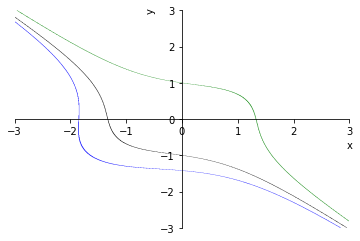
\includegraphics[width=0.6\textwidth]{./cap_edo1ordem/dados/fig_ex_edo1ordem_exata/fig_ex_edo1ordem_exata}
    \caption{Exemplo \ref{ex:edo1ordem_exata}. Esboços da solução geral para: (azul) $c=-10$, (preto) $c=-5$, (verde) $c=5$.}
    \label{fig:ex_edo1ordem_exata}
  \end{figure}
  
  \ifispython
  No \python, podemos computar a solução geral da EDO com os seguintes códigos:
\begin{verbatim}
In : from sympy import *
...: y = Function('y')
...: x,C1 = symbols('x,C1')
...: edo = 3*x**2-2*x*y(x)+2 + (6*y(x)**2-x**2+3)*diff(y(x),x)
...: sg = dsolve(edo, y(x), simplify=False)
...: sg
Out: Eq(x**3 - x**2*y(x) + 2*x + 2*y(x)**3 + 3*y(x), C1)
\end{verbatim}
  Os esboços dos gráficos podem ser obtidos com:
\begin{verbatim}
In : var('y')
...: sg = sg.subs(y(x),y)
...: p = plot_implicit(sg.subs(C1,-10), (x,-3,3), (y,-3,3),
...:          line_color="blue", show=False)
...: q = plot_implicit(sg.subs(C1,-5), (x,-3,3), (y,-3,3),
...:          line_color="black", show=False)
...: p.extend(q)
...: q = plot_implicit(sg.subs(C1,5), (x,-3,3), (y,-3,3),
...:          line_color="green", show=False)
...: p.extend(q)
...: p.show()
\end{verbatim}
  \fi
\end{ex}

\subsection{Método dos fatores integrantes}

Para algumas equações
\begin{equation}\label{eq:eqnexata}
  {\color{blue}M(x,y) + N(x,y)\frac{dy}{dx} = 0}
\end{equation}
não exatas é possível aplicar o método dos fatores integrantes para convertê-las em equações exatas.

A ideia é buscar por um fator integrante $\mu = \mu(x,y)$ tal que
\begin{equation}
  {\color{blue}\mu M(x,y) + \mu N(x,y)\frac{dy}{dx} = 0}
\end{equation}
seja uma equação exata, i.e.
\begin{equation}
  \frac{\p}{\p y}\left(\mu M(x,y)\right) = \frac{\p}{\p x}\left(\mu N(x,y)\right).
\end{equation}
Ou seja, $\mu$ deve ser tal que
\begin{gather}
  \frac{\p}{\p y}\left(\mu M(x,y)\right) - \frac{\p}{\p x}\left(\mu N(x,y)\right) = 0 \\
  \mu_y M + \mu M_y - \mu_x N - \mu N_x = 0.
\end{gather}
Com isso, pode-se concluir que $\mu = \mu(x,y)$ deve satisfazer
\begin{equation}\label{eq:eqexata_fatorint}
  {\color{blue}M\mu_y - N\mu_x + (M_y - N_x)\mu = 0}.
\end{equation}

Em geral, resolver \eqref{eq:eqexata_fatorint} pode ser tão ou mais difícil que resolver a EDO original \eqref{eq:eqnexata}. Vejamos alguns casos em que é possível encontrar o fator $\mu$.

\subsubsection{$\pmb{\mu = \mu(x)}$}

No caso de $\mu = \mu(x)$ (função de $x$ apenas), a equação \eqref{eq:eqexata_fatorint} resume-se a
\begin{equation}\label{eq:eqnexata_fatorintx}
  {\color{blue}\frac{d\mu}{dx} = \frac{M_y-N_x}{N}\mu}.
\end{equation}
Ou seja, se
\begin{equation}
  \frac{M_y-N_x}{N}
\end{equation}
é função apenas de $x$, então podemos calcular um fator integrante $\mu = \mu(x)$ resolvendo a EDO linear \eqref{eq:eqnexata_fatorintx}.

\begin{ex}\label{ex:edo1ordem_exata_fix}
  Vamos resolver a EDO
  \begin{equation}\label{eq:nexata_fatintx}
    (x+2)\sen(y) + x\cos(y)\frac{dy}{dx} = 0.
  \end{equation}
  Denotando
  \begin{align}
    M(x,y) &= (x+2)\sen(y) \\
    N(x,y) &= x\cos(y)
  \end{align}
  vemos que
  \begin{equation}
    \frac{\p}{\p y}M(x,y) = (x+2)\cos(y) \neq \cos(y) = \frac{\p}{\p x}N(x,y).
  \end{equation}
  Ou seja, não é uma equação exata. Por outro lado,
  \begin{align}
    \frac{M_y-N_x}{N} &= \frac{(x+2)\cos(y) - \cos(y)}{x\cos(y)} \\
                      &= \frac{x+1}{x}
  \end{align}
  é função apenas de $x$, o que nos indica a existência de um fator integrante $\mu = \mu(x)$ satisfazendo a seguinte EDO linear
  \begin{equation}
    \frac{d}{dx}\mu = \frac{M_y-N_x}{N}\mu. 
  \end{equation}
  Ou seja, resolvemos
  \begin{gather}
    \frac{d\mu}{dx} = \frac{x+1}{x}\mu \\
    \frac{1}{\mu}\,d\mu = \frac{x+1}{x}\,dx \\
    \ln|\mu| = x + \ln|x| + c \\
    \mu = cxe^x.
  \end{gather}

  Com isso, escolhendo o fator integrante $\mu = xe^x$ a equação
  \begin{equation}\label{eq:nexata_fatintx_aux}
    \mu M + \mu N\frac{dy}{dx} = 0
  \end{equation}
  é exata e é equivalente a EDO \eqref{eq:nexata_fatintx}. De fato, temos
  \begin{align}
    \frac{\p}{\p y}(\mu M) &= \frac{\p}{\p y}\left[(x^2+2x)e^x\sen(y)\right] \\
                           &= (x^2+2x)e^x\cos(y) \\
                           &= \frac{\p}{\p x} \left[x^2e^x\cos(y)\right] \\
                           &= \frac{\p}{\p x}(\mu N).
  \end{align}

  Para resolver \eqref{eq:nexata_fatintx_aux}, buscamos por uma função $\Psi = \Psi(x,y)$ tal que
  \begin{gather}
    \frac{\p}{\p y}\Psi(x,y) = \mu N \\
    \Psi(x,y) = \int x^2e^x\cos(y)\,dy + f(x) \\
    \Psi(x,y) = x^2e^x\sen(y) + f(x).
  \end{gather}
  Bem como, $\Psi$ deve satisfazer
  \begin{gather}
    \frac{\p}{\p x}\Psi(x,y) = \mu M \\
    (x^2 + 2x)e^x\sen(y) + f'(x) = (x^2 + 2x)e^x\sen(y) \\
    f'(x) = 0 \\
    f(x) = c.
  \end{gather}

  Logo, podemos concluir que a solução geral de \eqref{eq:nexata_fatintx}  é dada por
  \begin{equation}\label{eq:ex_edo1ordem_exata_fix_sol}
    x^2e^x\sen(y) = c.  
  \end{equation}

  \ifispython
  No \python, podemos computar a solução geral com:
\begin{verbatim}
In : from sympy import *
...: y = Function('y')
...: x,C1 = symbols('x,C1')
...: edo = (x+2)*sin(y(x))+x*cos(y(x))*diff(y(x),x)
...: sg = dsolve(edo, y(x), simplify=False)
...: sg
Out: Eq(log(cos(y(x))**2 - 1)/2, C1 - x - 2*log(x))
\end{verbatim}
  Esta solução é equivalente a \eqref{eq:ex_edo1ordem_exata_fix_sol}?
  \fi
\end{ex}

\ifispython
\begin{obs}
  A função \verb+checkodesol+ do \sympy permite verificar se uma expressão/equação é solução de uma dada EDO. No caso de exemplo anterior (Exemplo \ref{ex:edo1ordem_exata_fix}), podemos verificar a solução \eqref{eq:ex_edo1ordem_exata_fix_sol} com o seguinte código:
\begin{verbatim}
In : from sympy import *
...: y = Function('y')
...: x,C1 = symbols('x,C1')
...: edo = (x+2)*sin(y(x))+x*cos(y(x))*diff(y(x),x)
...: sol = Eq(x**2*exp(x)*sin(y(x)),C1)
...: checkodesol(edo,sol)
Out: [(True, 0), (True, 0)]
\end{verbatim}
\end{obs}
\fi

\subsubsection{$\pmb{\mu = \mu(y)}$}

No caso de $\mu = \mu(y)$ (função de $y$ apenas), a equação \eqref{eq:eqexata_fatorint} resume-se a
\begin{equation}\label{eq:eqnexata_fatorinty}
  {\color{blue}\frac{d\mu}{dy} = \frac{N_x-M_y}{M}\mu}.
\end{equation}
Ou seja, se
\begin{equation}
  \frac{N_x-M_y}{M}
\end{equation}
é função apenas de $y$, então podemos calcular um fator integrante $\mu = \mu(y)$ resolvendo a EDO linear \eqref{eq:eqnexata_fatorinty}.

\begin{ex}
  Vamos resolver a EDO
  \begin{equation}\label{eq:ex_nexata_fatinty}
    y + (2x - ye^y)\frac{dy}{dx} = 0.
  \end{equation}
  Denotando
  \begin{align}
    M(x,y) &= y \\
    N(x,y) &= 2x - ye^y
  \end{align}
  vemos que
  \begin{equation}
    \frac{\p}{\p y}M(x,y) = 1 \neq 2 = \frac{\p}{\p x}N(x,y).
  \end{equation}
  Ou seja, não é uma equação exata. Por outro lado,
  \begin{equation}
    \frac{N_x-M_y}{M} = \frac{1}{y}
  \end{equation}
  é função apenas de $y$. Com isso, podemos obter um fator integrante $\mu = \mu(y)$ resolvendo a seguinte EDO linear
  \begin{gather}
    \frac{d\mu}{dy} = \frac{N_x-M_y}{M}\mu \\
    \frac{d\mu}{dy} = \frac{1}{y}\mu \\
    \frac{1}{\mu}\,d\mu = \frac{1}{y}\,dy \\
    \ln|\mu| = \ln|y| + c \\
    \mu = cy.
  \end{gather}

  Desta forma, podemos escolher o fator integrante $\mu = y$ de forma que a equação
  \begin{equation}\label{eq:ex_exata_fatinty}
    \mu M + \mu N\frac{dy}{dx} = 0
  \end{equation}
  é exata e equivalente a EDO \eqref{eq:ex_nexata_fatinty}. De fato, temos
  \begin{align}
    \frac{\p}{\p y}(\mu M) &= \frac{\p}{\p y}(y^2) \\
                           &= 2y \\
                           &= \frac{\p}{\p x}\left[(2x-ye^y)y\right] \\
                           &= \frac{\p}{\p x}(\mu N).
  \end{align}
  
  Sendo \eqref{eq:ex_exata_fatinty} uma equação exata, buscamos por uma função $\Psi = \Psi(x,y)$ tal que
  \begin{gather}
    \frac{\p}{\p x}\Psi(x,y) = \mu M(x,y) \\
    \Psi(x,y) = \int y^2\,dx + f(y) \\
    \Psi(x,y) = xy^2 + f(y).
  \end{gather}
  Bem como,
  \begin{gather}
    \frac{\p}{\p y}\Psi(x,y) = \mu N(x,y) \\
    2xy + f'(y) = 2xy - y^2e^{y} \\
    f'(y) = -y^2e^{y} \\
    f(y) = -(y^2-2y+2)e^y + c.
  \end{gather}

  Logo, concluímos que a solução geral da EDO \eqref{eq:ex_nexata_fatinty} é
  \begin{equation}
    xy^2 - (y^2-2y+2)e^y = c.
  \end{equation}

  \ifispython
  Vamos verificar esta solução no \python:
\begin{verbatim}
from sympy import *
y = Function('y')
x,C1 = symbols('x,C1')
edo = y(x)+(2*x-y(x)*exp(y(x)))*diff(y(x),x)
sol = Eq(x*y(x)**2-(y(x)**2-2*y(x)+2)*exp(y(x)),C1)
checkodesol(edo,sol,func=y(x),solve_for_func=False)
\end{verbatim}
  Tendo em vista que o \sympy\;não resolve esta EDO diretamente, a opção \verb+solve_for_func=False+ foi utilizada para impedir que o \sympy\;tente resolver a EDO.
  \fi
\end{ex}

\subsection*{Exercícios resolvidos}

\begin{exeresol}
  Verifique se a EDO
  \begin{equation}
    x^2 + (2xy-y^2)\frac{dy}{dx} = -y^2
  \end{equation}
  é exata. Caso não seja, busque por um fator integrante para reescrevê-la como uma equação exata.
\end{exeresol}
\begin{resol}
  Para verificarmos se a equação é exata, vamos colocá-la reescrevê-la na seguinte forma
  \begin{equation}
    x^2 + y^2 + (2xy-y^2)\frac{dy}{dx} = 0.
  \end{equation}
  Com isso, identificamos
  \begin{align}
    M(x,y) &= x^2 + y^2,\\
    N(x,y) &= 2xy-y^2.
  \end{align}
  Ainda, temos
  \begin{equation}
    \frac{\p M}{\p y} = 2y
  \end{equation}
  e
  \begin{equation}
    \frac{\p N}{\p x} = 2y.
  \end{equation}
  Como
  \begin{equation}
    \frac{\p M}{\p y} = \frac{\p N}{\p x},
  \end{equation}
  concluímos que a EDO é exata.
\end{resol}

\begin{exeresol}
  Resolva o seguinte PVI:
  \begin{align}
    &sen(y) + (x\cos(y)+1)\frac{dy}{dx} = 0,\\
    &y(0)=\pi.
  \end{align}
\end{exeresol}
\begin{resol}
  Denotando
  \begin{equation}
    M(x,y) = \sen(y),\quad N(x,y) = x\cos(y)+1,
  \end{equation}
  vemos que a EDO associada ao PVI é uma equação exata. Logo, para resolvê-la buscamos por uma função $\Psi = \Psi(x,y)$ tal que
  \begin{gather}
    \frac{\p \Psi}{\p x} = M(x,y) \\
    \Psi = \int M(x,y)\,dx + f(y) \\
    \Psi = x\sen(y) + f(y).
  \end{gather}
  Bem como, $\Psi$ deve ser tal que
  \begin{gather}
    \frac{\p}{\p y}\Psi(x,y) = N(x,y) \\
    x\cos(y) + f'(y) = x\cos(y)+1 \\
    f'(y) = 1 \\
    f(y) = y + c.
  \end{gather}
  Logo, a solução geral da EDO associada é dada por
  \begin{equation}
    x\sen(y) + y = c.
  \end{equation}

  Por fim, aplicando a condição inicial $y(0) = 1$, obtemos
  \begin{gather}
    0\cdot\sen(1)+1 = c \\
    c = 1.
  \end{gather}
  Concluímos que a solução do PVI é dada por
  \begin{equation}
    x\sen(y) + y = 1.
  \end{equation}
\end{resol}

\subsection*{Exercícios}

\begin{exer}
  Verifique se a seguinte EDO é exata. Justifique sua resposta.
  \begin{equation}
    \frac{dy}{dx} = \frac{\cos(y)}{1+x\sen(y)}.
  \end{equation}
\end{exer}
\begin{resp}
  Exata
\end{resp}

\begin{exer}
  Resolva a seguinte EDO
  \begin{equation}
    \cos(y) + (1-x\sen(y))\frac{dy}{dx} = 0.
  \end{equation}
\end{exer}
\begin{resp}
  $x\cos(y) + y = c$
\end{resp}

\begin{exer}
  Mostre que a seguinte EDO não é exata
  \begin{equation}
    xy^2+1 - x^2y\frac{dy}{dx} = 0.
  \end{equation}
  Ainda, mostre que o fator integrante $\mu = x^{-4}$ pode ser usado para transformar esta em uma equação exata. Por fim, resolva-a.
\end{exer}
\begin{resp}
  $-\frac{x^{-2}y^2}{2}-\frac{x^3}{3} = c$
\end{resp}

\begin{exer}
  Resolva a seguinte EDO
  \begin{equation}
    6xy+y^2 + (2x^2+xy)\frac{dy}{dx} = 0.
  \end{equation}
\end{exer}
\begin{resp}
  $(xy+2x^2)^2-4x^4=c$
\end{resp}

\begin{exer}
  Resolva o seguinte PVI
  \begin{equation}
    y + (y-3x)\frac{dy}{dx} = 0,\\
    y(1)=1
  \end{equation}
\end{exer}
\begin{resp}
  $xy^{-3}-\frac{y^{-2}}{2} = \frac{1}{2}$
\end{resp}